\section{Public stock and the value of additional computation}
\label{app:public-stock}
The frozen-transfer study in Appendix~\ref{app:rule-transfer} changes scoring
without teaching the policies the new games. We therefore run a separate
factorial study with rule-specific adaptation. Its question is whether public
information, an additional stock decision, or amplified continuation stakes
increase the benefit of computation. This is a comparison of search gains
within games, not an absolute ranking of strength across different games.

\paragraph{Three factors, eight games.}
Preview makes the next two stock cards visible before the hand action,
replenishing their visibility after each draw. Choice reveals two cards after
the hand action and capture, lets the player draw one, and retains the other
at the top. Without preview, the replacement remains hidden until the next
stock-choice phase; the retained card remains public. With both factors,
the player sees both options before selecting a hand card. At a yaku stop,
Stakes transfers $(S_w+S_\ell)2^{\mathbf{1}\{k_w>0\}}$ from loser to winner.
Each $S_i$ is that player's current captured-card score under paper8,
including their own declaration effects; $k_w$ counts the winner's
koi declarations. Captured sets are evaluated separately. The ordinary
one-point exhaustion settlement remains. All eight combinations retain the
original yaku, eight-round match, 30 initial points, bankruptcy and 16-turn round limit. A stock choice
adds a decision, not a turn or draw.

\paragraph{Adaptation and qualification.}
Two scratch-trained controls fail their quality gate, so the replacement
protocol freezes each of our two stronger parent actors and trains an
observation-only residual policy and critic. Each rule receives 4,194,304
additional decisions per parent, 67,108,864 in total. Inputs include the two
revealed cards and rule/phase flags; they exclude hidden hands, hidden stock
order and future randomness. Training counts are not strength measurements.

On 256 new duplicate streams, with both seats, the controls score 76.6602\%
and 79.6875\% against greedy play and 50.4883\% and 52.1484\% against
unassisted GPU-batched RL-WP. Both pass the prespecified 65\% greedy and
45\% WP gates. These 2,048 qualification matches are separate from the
historical assisted-2023 comparison and are replayed independently in Python.

\paragraph{Two fixed search protocols.}
The first screen uses 64 duplicate streams and 0/2/8/32 sampled worlds per
legal root action. It simulates 32 decisions under the fixed adapted policies,
then uses the adapted observation-only critic. All root actions share sampled
worlds; the baseline action is retained unless another action's mean paired
advantage exceeds one estimated standard error. Worlds preserve public stock
and the player's own cards but use a uniform deal-consistent hidden proposal,
not an action-conditioned posterior.

A separate protocol completes the current round before evaluating its leaf.
For each fixed policy/rule, it computes a table of expected terminal utility
before a fresh deal, indexed by round, absolute dealer and player-0 points.
Backward computation uses 512 conditional round rollouts per live cell,
483,328 per model. All sixteen tables are complete: 7,733,248 conditional
rounds and 163,572,208 transitions. Absolute dealer remains necessary because the released
parent encoder observes seat identity. Lookup uses only the public boundary;
the next hidden deal is not used. Every saved target and table mean is reduced
independently, with four fixed samples per cell replayed in Python (3,776
rounds per table; 60,416 rounds and 1,276,957 decisions in total). These are
preparation rounds, not full evaluation matches.
The second screen reuses the same sixteen policies, with no new training,
on 32 separate duplicate streams at 0/8/32/128 worlds per action and a
2.5-standard-error guard. Failure to finish a rollout round is an error;
there is no neural-value cutoff. Every scored match in both screens is
replayed in Python.

\paragraph{Selection and scope.}
Each screen selects the noncontrol rule with the largest worse-parent
high-budget gain over its own no-search actor. Advancement requires positive
gains for both parents and a worse-parent gain above the control's. Reserved
confirmation uses 512 new duplicate streams for the first protocol and 128
for the second. Each requires four positive one-sided 98.75\% paired-bootstrap
lower bounds: a positive selected-rule gain and a positive difference from
the control's gain for each parent. This familywise target is per protocol;
no across-protocol multiplicity adjustment is claimed. Failed cohorts are
neither extended nor pooled. All rule curves, including nonmonotonic effects,
must be reported.
Confirmation compares the selected rule with control; rankings against
the remaining rules remain exploratory. Equal adaptation budgets need not
produce equally mature policies; larger gains can partly reflect remaining
policy errors. Conclusions therefore concern this fixed training/search regime.

\paragraph{First-screen result.}
The 32-decision screen completes 8,192 matches, 55,032 rounds and 1,153,925
policy decisions on its 64 shared duplicate streams. All scored decisions
pass Python replay; independent reductions reproduce scores and evaluated-match counters.
Search uses 22,993,192 rollouts and 665,914,496 transitions. The all-three
rule has the largest worse-parent gain: 33.5938 and 28.1250 percentage points,
versus control changes of $-10.5469$ and $-9.7656$ points. Preview plus choice
scores slightly higher for parent 1, so this selection is not a claim of
uniform superiority. Every rule loses mean score at two worlds. The reserved
512-stream confirmation is reported separately below.
At 32 worlds, all-three matches average 5.16/5.10 rounds, versus 7.51/7.52
for preview plus choice. The work comparison therefore includes different
match lengths, as well as different policies and decision spaces.

\begin{table}[ht]
\centering
\small
\begin{tabular}{lrrrr}
\toprule
Rule & $1\times$ & $4\times$ & $16\times$ & $16\times$ work \\
\midrule
Control & -16.02/-22.66 & -13.28/-17.97 & -10.55/-9.77 & 241.6/236.8 \\
Stakes & -21.09/-26.56 & -24.22/-14.06 & -3.12/-12.50 & 170.2/178.9 \\
Choice & -30.08/-22.27 & -14.84/+0.39 & +14.45/+7.03 & 345.3/330.4 \\
Choice + stakes & -25.39/-16.02 & -7.03/+3.12 & +17.19/+17.97 & 273.8/239.0 \\
Preview & -8.20/-14.06 & -0.39/-2.73 & +14.84/+11.72 & 237.3/236.5 \\
Preview + stakes & -13.28/-8.98 & -6.64/+3.52 & +12.50/+15.23 & 174.1/173.1 \\
Preview + choice & -9.77/-18.36 & +10.94/+2.34 & +26.17/+29.30 & 331.4/338.8 \\
All three & -10.55/-22.66 & +8.98/+6.64 & +33.59/+28.12 & 230.2/227.8 \\
\bottomrule
\end{tabular}

\caption{Complete first-screen curves. Entries are parent-0/parent-1 gains in
percentage points over the no-search actor. The nominal budgets are 2, 8 and
32 worlds per legal action; horizon is 32 decisions. Work is thousands of
physical search transitions per actual match, excluding policy training.
Nominal particle ratios do not match costs across games. All eight rules
share 64 duplicate streams; their 8,192 matches are not independent streams.}
\label{tab:public-stock-v2-curves}
\end{table}

\paragraph{Completed-round screen.}
The second screen completes 4,096 matches, 27,752 rounds and 574,620 scored
and replayed decisions on 32 shared duplicate streams. It uses 46,309,552
rollouts and 653,460,580 online transitions, separately from table preparation.
Preview plus choice gains 36.7188/34.3750 points at 128 worlds, compared with
control changes of $-3.1250/+3.1250$ points. Its worse-parent gain ties
all three; the registered lexicographic tie-break selects preview plus choice.
This is not a confirmed ranking between those alternatives. Increasing eight
to 128 worlds adds 21.8750/20.3125 points within the selected rule in development.
The reserved 128-stream confirmation is reported below.

\begin{figure}[ht]
\centering
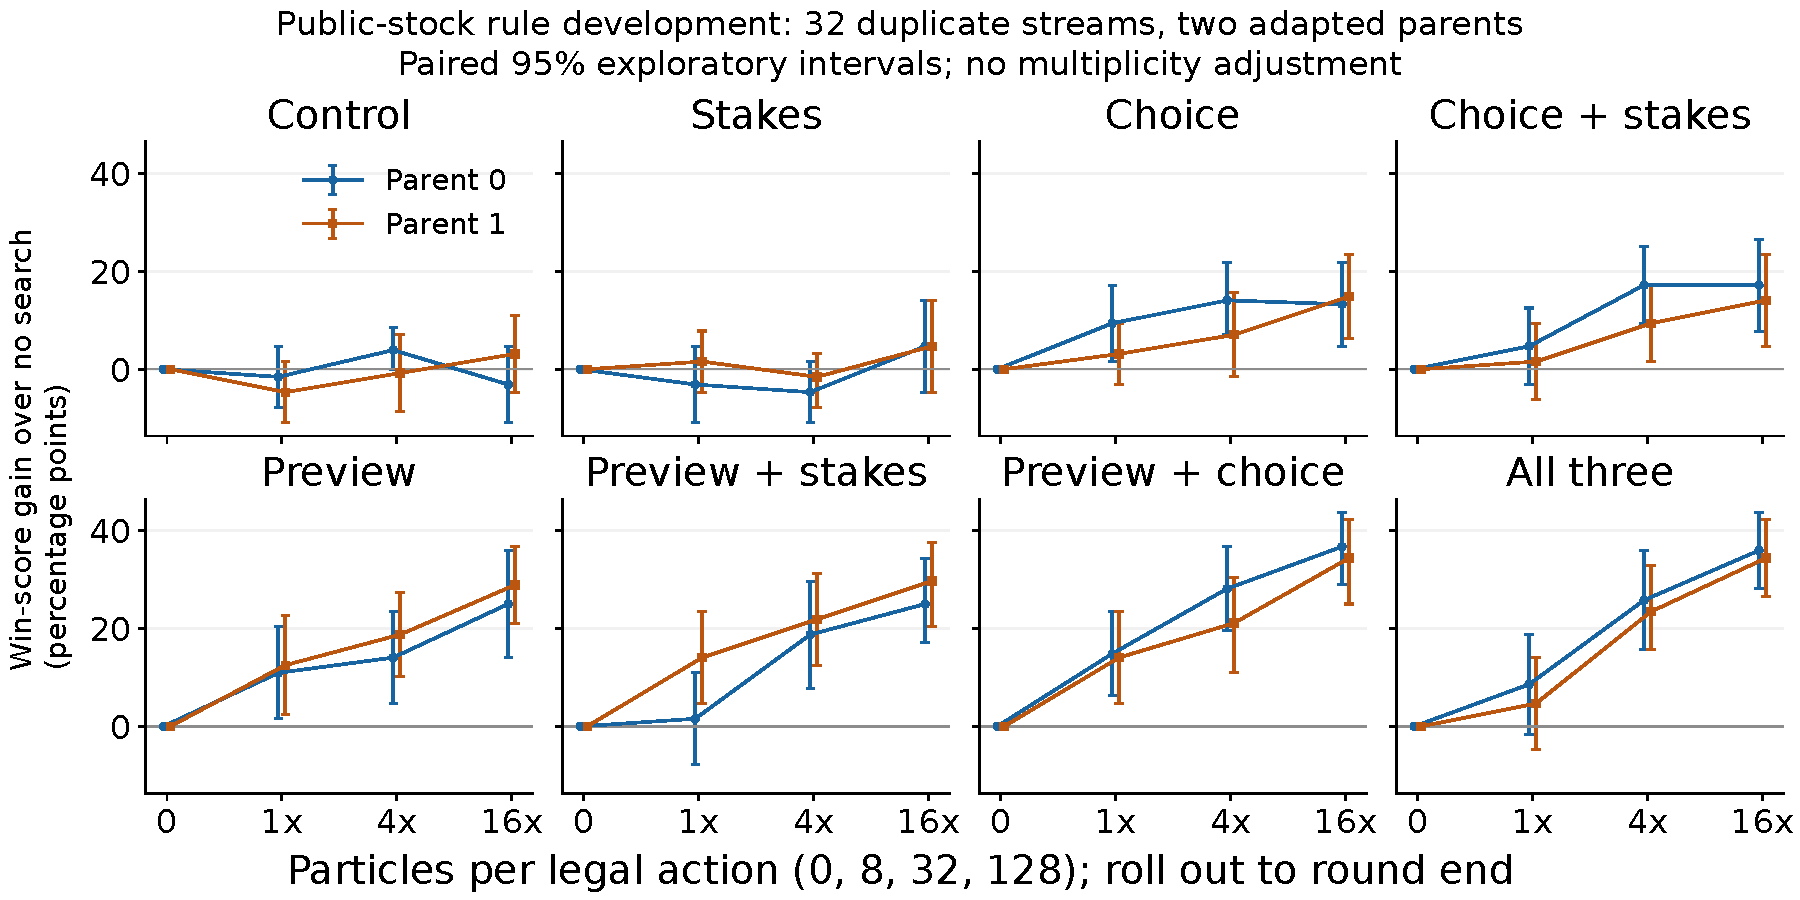
\includegraphics[width=\linewidth]{generated/public_stock_v3/public_stock_scaling.pdf}
\caption{Completed-round development curves. Each rule uses its own
adapted no-search actor as opponent. Intervals are exploratory paired 95\%
intervals on 32 duplicate streams, without multiplicity or selection adjustment.
The nominal budgets are 8, 32 and 128 worlds per legal root action; actual
work varies across rules. These intervals are not the confirmation criterion.}
\label{fig:public-stock-v3-curves}
\end{figure}

\FloatBarrier
\paragraph{Independent confirmations.}
Both registered four-inequality criteria pass (Table~\ref{tab:public-stock-confirmation}).
The first confirmation contains 16,384 matches, 112,112 rounds and 2,249,011
replayed decisions on 512 new duplicate streams; it uses 45,492,908 rollouts
and 1,313,528,021 online transitions. The second contains 3,072 matches,
23,850 rounds and 492,836 replayed decisions on 128 separate new streams,
using 42,932,832 rollouts and 605,313,887 transitions. Independent reductions
reproduce scores, match counts, rounds and scored decisions. Search work is
recorded separately. These cohorts are neither pooled nor extended.

\begin{table}[ht]
\centering\small
\begin{tabular}{llrrr}
\toprule
Search & Parent & Score (\%) & Gain [LB] & Excess [LB] \\
\midrule
32 decisions & 0 & 82.47 & +32.47 [+29.93] & +41.85 [+37.84] \\
32 decisions & 1 & 80.91 & +30.91 [+28.12] & +38.67 [+34.62] \\
Round end & 0 & 85.16 & +35.16 [+30.66] & +32.03 [+25.78] \\
Round end & 1 & 85.16 & +35.16 [+30.47] & +31.64 [+25.59] \\
\bottomrule
\end{tabular}

\caption{Held-out selected-rule results. Gain is the high-budget change from
no search; excess subtracts the corresponding control gain. Changes are in
percentage points; brackets give one-sided 98.75\% paired-bootstrap lower
bounds. Four positive lower bounds are required within each protocol.
The first selects all three factors; the second selects preview plus choice.
Each system faces its own adapted no-search actor; scores count ties as one half.}
\label{tab:public-stock-confirmation}
\end{table}

For preview plus choice, increasing eight to 128 worlds improves score by
22.85 points for parent 0 (secondary paired 95\% interval 17.19--28.52) and
17.77 points for parent 1 (11.72--23.83). Additional computation therefore
helps beyond the first nonzero budget in this held-out regime. It need not
help at every budget: the first protocol's two-world scores remain below
50\% for both selected-rule parents (30.86/33.45\%).

These sampled searches do not inherit the exact improvement guarantee of the
main method. Uniform beliefs can be misspecified, and table errors propagate
across rounds; conditional table standard errors do not cover that propagated
uncertainty. The two protocols also differ in guard and budgets, so their
comparison cannot isolate the effect of caching. Increasing particles increases
sampled worlds, not the fixed rollout horizon. Particle counts do not equalize
work across rules. Offline preparation, online transitions and
wall time must remain distinct. The results establish a reproducible
computation benefit for fixed adapted systems, not maximal strength or a
confirmed ranking between the two selected rules. Changed opponents,
stronger adaptation and matched work allowances are follow-up tests.
